\chapter{Gradient and categorical aspects of wordlikeness judgements}
\label{gradience}

\citet{Chomsky1965} observe that speakers internalize not only generalizations governing phonological alternations in their language, but also about the shapes of possible words in their language. \citeauthor{Chomsky1965} illustrate this latter type of knowledge with two nonce words *\emph{blick} [blɪk] and *\emph{bnick} [bnɪk]; whereas \emph{blick} is a possible word of English, \emph{bnick} can be immediately recognized not only as unattested but also impossible.

What is peculiar about 

% actually a mystery
% follows from syllabification

The problems of this account have 

Richer representations in 

the increasingly rich representations in 

A number of innovations 

The requirement that 

Citing the presence of epenthesis in loanword adaptation, \citet{Hooper1973} 



%\citet{Hooper1973} is an early proponent of introducing syllable representations into generative phonology; citing loanword adaptation process, she writes they ``show that syllable-formation is productive, and that there is very possibly a rule that inserts V's into syllables in the correct position.'' \citep[][101-102]{Hooper1973}. 
%\citet{Kiparsky1982b} also recognizes that the requirement that outputs be syllabifiable may derive generalizations about the shape of possible morphs. % presumably by Stampean occultation %(for which Kiparsky cites \citealt{McCarthy1979b})


%\citet{Ito1989a}
%\citet{Noske1992}
%s unsyllabifiable outputs \citep[e.g.][]{Ito1989a,Noske1992}, then \emph{bnick} is an impossible output, doomed to be modified (perhaps to \emph{nick}; \citealt[][19f.]{Wolf2009}), and /bnɪk/ is an impossible UR by Stampean occultation.

Others have suggested that cluster simplification might result: \citet[][19f.]{Wolf2009}, for instance, proposes that /bnɪk/ would be realized [nɪk].

\citep[e.g.,][]{Pertz1975,Albright2007}


% fails gradience

\begin{quote}
A defect of current grammatical acounts of phonotactics is that they render simple up-or-down- decisions concerning well-formedness and cannot account for gradient judgements. But when judgements are elicited in a controlled fashion from speakers, they always emerge as gradient, including all intermediate values. \citep[][371]{Shademan2006}

In the particular domain of phonotactics gradient intuitions are pervasive: they have been found in every experiment that allowed participants to rate forms on a scale.
\citep[][382]{Hayes2008a}

When native speakers are asked to judge made-up (nonce) words, their intuitions are rarely all-or-nothing. In the usual case, novel items fall along a gradient cline of acceptability. \citep[][9]{Albright2009a}
\end{quote}

%\ldots{}we consider the ability to model gradient intuitions to be an important criterion for evaluating phonotactic models. \citep[][382]{Hayes2008a}
%If adhered to literally, however, the gradience hypothesis becomes an axiom.

\section{The gradience hypothesis}

The gradience hypothesis, as defined below, has both weak and strong forms.

% weak version
% strong version
\subsection{A brief history}
\subsubsection{In syntax}
% LSLT
% Aspects
% CH
% LGB
\subsubsection{In phonology}
% SPR
% GH
% CH
% SPE
% Borowsky
\subsubsection{The last two decades}
% OT/HG
% Coleman 1997
\subsection{Ontology}
% intro text
\subsubsection{Representational likelihood}
% C&P, positional probs, bigrams
\subsubsection{Gradient wellformedness}
% hayes & wilson, anttilla, coetzee & pater
\subsubsection{Lexical similarity}
% greenberg & jenkins, ohala & ohala, bailey & hahn
\subsection{Falsifiability}
% considers how one might falsify
\subsubsection{Against an axiomatic interpretation}
% not an axiom: hayes & wilson
\subsubsection{The weak hypothesis}
% \citet{Armstrong1983}
% schutze quote
% stuff about mathcog
\subsubsection{The strong hypothesis}
% comparison of gradient models
% incremental contribution of gradient models
\section{Evaluation}

The strong gradience hypothesis can only be evaluated by comparing individual gradient models to actual wordlikeness data. The remainder of this chapter describes such a study using state-of-the-art phonotactic models and data from English.

\subsection{Data sources}

The evaluation makes exclusive use of previously published wordlikeness data sets. To be included in this evaluation, a study must have the three following characteristics. First, the stimuli must consist only of monomorphs presented auditorily. Secondly, a significant portion of the stimuli must contain gross phonotactic violations (e.g., *\emph{bnick}), and finally, the ratings, averaged across subjects, must be publicly available. The study by \citet{Bailey2001} which is ineligible because very few stimuli contain phonotactic violations, and the studies by \citet{Shademan2007} is not considered here because the data is not available to the public.

\subsubsection{\citealt{Greenberg1964}}

\citet{Greenberg1964} investigated wordlikeness using the technique of free magnitude estimation, a mechanism which has become increasingly popular among syntactians \citep[e.g.,][]{Bard1996}. At the beginning of the experiment, the subject heard a recording of the word \emph{stick}. In subsequent trials, the subjects heard a new (possibly nonce) word and is asked to report ``how far would you say that is from English?'', with \emph{stick} at ``1''; subjects are told that a word that is ``twice as far from English'' as \emph{stick} should be scored ``2''. The data used here are from \citeauthor{Greenberg1964}'s Experiment B, in which 17 undergraduates were presented 17 stimuli in all. In addition to \emph{stick}, several other English words were included in the stimuli; these four items were excluded from further analyses, leaving 13 stimuli. As is standard practice in psychophysics \citep[e.g,]{Butler1987}, these magnitude ratings were log-transformed before analysis.

\subsubsection{\citealt{Scholes1966}}

\citet{Scholes1966} conducted a number of English wordlikeness judgement with middle school children. The data used here come from his ``experiment 5'', in which 63 monosyllabic items were presented to 33 seventh-grade students. For each stimulus, the subjects produced forced choice ``yes''/``no'' answers to the question of whether the item ``is likely to be usable as a word of English''. \citet{Hayes2008a} and \citet{Albright2009a} analyse this data as gradient by performing an item averaging using the fraction of ``yes'' answers for each stimulus. For instance, 22 of the 33 students answered ``yes'' for \emph{shlerk} [ʃlɚk], so it is assigned a score of $0.666$. These stimuli are all ostensibly non-words, but include \emph{clung} [klʌŋ], the preterite and past participle of the verb \emph{cling}, and \emph{brung} [brʌŋ], a dialectical past participle for \emph{bring}. These two words were excluded and the remaining 61 stimuli were submitted to analysis. 

\subsubsection{\citealt{Albright2003b}}

\citet{Albright2003b} gathered wordlikeness judgements to serve as norms for a \emph{wug}-test. 87 items were presented to 20 undergraduate subjects, who rated each word on a seven-point Likert scale. The lowest point on the scale was labeled ``completely bizarre, impossible as an English word'', and that the highest point was labeled ``complete normal, would make a fine English word''.

\subsection{Model comparison}

These models are compared against wordlikeness ratings using non-parametric rank correlation statistics. While the use of the Pearson correlation is standard in the phonotactics literature, rank correlation statistics make none of the troublesome assumptions associated with this former method. The Spearman $\rho$ is most widely known rank correlation statistic, but the Kendall $\tau_b$ and Goodman-Kruskal $\gamma$ have much simpler interpretations, relating to the probabilities of {concordant} and {discordant} pairs \citep{Noether1981}. Consider the case here, in which model scores are compared with wordlikeness ratings. If a model predicts that *\emph{dresp} [?] is more highly rated than *\emph{srest}, this pair is {concordant} if speakers also rate *\emph{dresp} more English-like than *\emph{srest} and it is discordant if *\emph{srest} is rated more English-like. Both $\tau_b$ and $\gamma$ are based on ratios of the number of concordant and discordant pairs, differing only in their treatment of ``ties'' (in which, e.g., *\emph{dresp} and *\emph{srest} are scored the same, or rated the same); $\tau_b$ includes a correction for ties, whereas $\gamma$ discards tied pairs. Much like the familiar Pearson correlation, $\rho$, $\tau_b$ and $\gamma$ are all in the range [-1, 1]. The correlations of the four models, discussed below, are given in Table \ref{cor}.

\begin{table} \label{cor}
\centering
\begin{tabular}{l l l l l}
\toprule
Spearman $\rho$          & binary           & MaxEnt  & bigram           & density          \\
\midrule
\citealt{Greenberg1964}  & {0.845}          & {0.765} & {\textbf{0.863}} & {0.648}          \\
\citealt{Scholes1966}    & {0.791}          & {0.762} & {\textbf{0.827}} & {0.827}          \\
\citealt{Albright2003b}  & {0.725}          & {0.429} & {0.708}          & {\textbf{0.742}} \\
\midrule
Kendall $\tau_b$         & binary           & MaxEnt  & bigram           & density          \\
\midrule
\citealt{Greenberg1964}  & {\textbf{0.716}} & {0.585} & {0.692}          & {0.462}          \\
\citealt{Scholes1966}    & {\textbf{0.664}} & {0.597} & {0.652}          & {0.565}          \\
\citealt{Albright2003b}  & {\textbf{0.599}} & {0.343} & {0.506}          & {0.556}          \\
\midrule
Goodman-Kruskal $\gamma$ & bigram           & MaxEnt  & bigram           & density          \\
\midrule
\citealt{Greenberg1964}  & {\textbf{1.000}} & {0.684} & {0.692}          & {0.462}          \\
\citealt{Scholes1966}    & {\textbf{0.995}} & {0.634} & {0.667}          & {0.614}          \\
\citealt{Albright2003b}  & {\textbf{0.953}} & {0.656} & {0.509}          & {0.575}          \\
\bottomrule
\end{tabular}
\caption{Rank correlations between wordlikeness ratings and phonotactic models surprisingly reveal that the binary baseline meeds or exceeds the coverage of three state-of-the-art phonotactic models. All correlations are significant at $p = 0.05$.}
\end{table}

\subsubsection{Binary baseline}

The binary baseline here corrresponds to the null hypothesis that there are no gradient effects in wordlikeness judgements. To create such a baseline, it is necessary to distinguish between nonce words which contain a gross phonotactic violation and those which do not. Since all the observed phonotactic violations in the data can either be localized to the onset or rime, this problem reduces to the problem of determining whether a nonce word consists of a valid onset and rime. Rather than making this partition in a way based on any theoretical insights, the binary baseline is further ``cursed'' with the inability to abstract beyond seen data: any word which contains an unattested onset or rime is marked invalid. Despite the simplistic nature of this model, it outperforms the gradient models described below in most contexts. Further comparison of this model and possible improvements are sketched in \S\ref{limitations}.

\subsubsection{Maximum Entropy phonotactics}

\citeauthor{Hayes2008a} (\citeyear{Hayes2008a}; henceforth H\&W) develop a sophisticated model of phonotactic grammaticality which estimates a probability distribution over phoneme sequences by weighing constraints according to the principle of maximum entropy. H\&W find that the predictions of their model are closely correlated with the \citet{Scholes1966} wordlikeness ratings. A direct replication of this evaluation was attempted using the software, the model parameters, and training data used by H\&W. Since the training of model is inherently stochastic, producing slightly different outcomes on each run, the lowest scoring of ten runs is reported (H\&W:396) though in general there is not a great deal of variation between individual runs. One limitation of this model is that it is not feasible to score whole words, as the number of constraints which must be inspected grows expontentially as their scope increases. Following H\&W and of \citet{Albright2009a}, who also applies the maximum entropy model to the \citet{Albright2003b} norms, the model is trained and scored only on stimulus onsets. However, as a consequence, the maximum entropy model performs particularly poorly on this data set, in which many stimuli contain phonotactic violations in the rime.

\subsubsection{Segment bigram probability}

The bigram probability of a sequence $ijk$ is simply the product of three probabilities: the probability of an sequence-initial $i$, the probability that $j$ follows $i$, and the probability that $k$ follows $j$.

\begin{unlabeledexample}
$\displaystyle \hat{p}(ijk) = p(i|\textrm{start}) \cdot p(j|i) \cdot p(k|j)$
\end{unlabeledexample}

\noindent Bigram models are widely used in natural language processing, and \citet{Albright2009a} considers their relevance to modeling wordlikeness judgements. While the focus of \citeauthor{Albright2009a}'s study is on developing a model which uses bigrams over phonological features rather than segments themselves, \citeauthor{Albright2009a}'s evaluation, which includes both the \citeauthor{Scholes1966} and \citeauthor{Albright2003b} data sets, finds an advantage for segmental bigrams. 

\citeauthor{Albright2009a} estimates bigram probabilities using familiar maximum likelihood method over types in the lexicon. The variant of segmental bigrams used here computes probabilities with a simple type of smoothing in which the count of every bigram (including those never observed) is incremented by one, a technique known as Laplacian, or ``add one'' smoothing. This has the desirable effect that no nonce word is ever assigned a zero probability, and produces in a small increase in the correlation between the \citeauthor{Albright2003b} wordlikeness norms compared with the maximum likelihood estimate (Table \ref{albrightimproved}). This model consistenly outperformed the positional probability probability models of \citet{Vitevitch2004} and \citet{Vaden2009}. The bigram model consistently performs well in all the evaluations, and has the highest Spearman correlation with the \citeauthor{Greenberg1964} and \citeauthor{Scholes1966}, and is frequently second place model to the binary baseline elsewhere.

\begin{table} \label{albrightimproved}
\centering
\begin{tabular}{l r r r}
\toprule
                         & maximum likelihood & Laplacian smoothing \\
\midrule
Spearman $\rho$          & 0.660              & \textbf{0.708} \\
Kendall $\tau_b$         & 0.467              & \textbf{0.506} \\
Goodman-Kruskal $\gamma$ & 0.473              & \textbf{0.509} \\
\bottomrule
\end{tabular}
\caption{Laplacian smoothing increases the correlation between the segmental bigram model proposed by \citet{Albright2009a}, which uses maximum likelihood estimation, and the \citet{Albright2003b} wordlikeness norms. All correlations are significant at $p = 0.05$.}
\end{table}

\subsubsection{Lexical neighbors}

The hypothesis that wordlikeness judgements reflect similarity to known words has a long history and has been promoted by linguists as diverse as \citet{Greenberg1964}, \citet{Ohala1986b}, and \citet{Schutze2005}. There are now an extensive number of methods for computing similarity in the psycholinguistic literature. The simplest of these methods, neighborhood density \citep{Coltheart1977}, consistenly outperformed recent proposals by \citet{Bailey2001}, \citet{Vaden2009}, and \citet{Suarez2011}. \citeauthor{Coltheart1977} define the neighborhood density as the number of real monomorphemic words which can be changed into the target nonce word by a single insertion, deletion, or substition. For instance, the neighbors of \emph{blick} include \emph{blink} (insertion), \emph{lick} (deletion) and \emph{black} (substitution). While many studies \citep[e.g.,][]{Bailey2001} report robust lexical similarity effects, it may be that these effects are diminished in the presence of gross phonotactic violations, since dnesity performs more poorly than the competing models.

\subsection{Discussion}
\label{2dis}

\subsubsection{The strong gradience hypothesis}

The evaluation provides overwhelming evidence that the gradient phonotactic models are closely correlated with the binary baseline, but no gradient model is reliably superior to the baseline. This is not sufficient, however, to rule out the strong gradience hypothesis, which predicts that even once gross phonotactic violatoins are controlled for, gradient models contribute additional information about speakers' judgements.

As an exploratory analysis, the densities of ratings from the three studies, linearly transformed to the interval [0, 1] and split according to the binary baseline, are shown in Figure \ref{density}. In all three studies, it is possible to discern a relatively sharp separation between valid and invalid clusters.

\begin{figure} \centering \label{density}
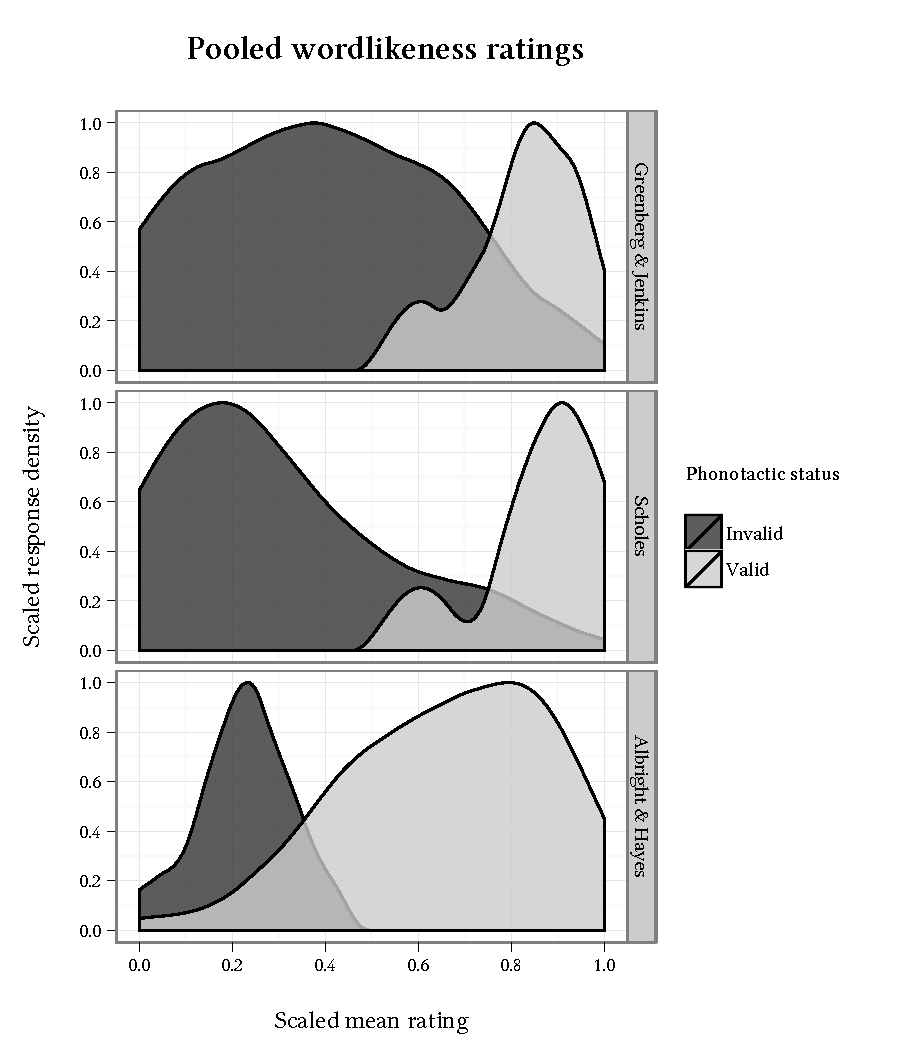
\includegraphics{density.pdf}
\caption{Average ratings of individual nonce words, linearly transformed to the interval [0, 1], tend to clump into two groups with little overlap; words which consist of  attested onsets and rimes receive ratings near ceiling, whereas ratings of phonotactically invalid words are spread across the lower half of the spectrum.}
\end{figure}

Figure \ref{density} also reveals intermediate ratings are used. The weak gradience hypothesis requires a demonstration that these intermediate ratings are correlated once the categorical effects are taken into account. The residual contribution of the three gradient models is quantified in the following manner. Instead of calculating rank correlations directly on the model scores as in Table \ref{cor}, the model scores are mapped to ranks with the additional constraint that all ``valid'' stimlui are ranked higher than all ``invalid'' stimuli, and used to compute new correlation statistics. To estimate the improvement in correlation generating by augmenting the binary model with gradient predictions, the binary baseline correlation statistics from this number; these differences are given in \ref{controlled}.  In most cases, including the gradient models on top of the binary baseline results in a reduction of performance in stark contrast to the predictions of the strong gradience hypothesis.

\begin{table} \label{controlled}
\centering
\begin{tabular}{l r r r}
\toprule
Spearman $\rho$          & MaxEnt            & bigram            & density  \\
\midrule
\citealt{Greenberg1964}  & $-0.060$          &  \textbf{0.038} & $-0.017$ \\
\citealt{Scholes1966}    & $-0.029$          &  \textbf{0.047} & $-0.035$ \\
\citealt{Albright2003b}  & $-0.008$          & $-0.015$          & \textbf{0.018} \\
\midrule
Kendall $\tau_b$         & MaxEnt            & bigram            & density  \\
\midrule
\citealt{Greenberg1964}  & $-0.114$          & \textbf{$-$0.007} & $-0.084$ \\
\citealt{Scholes1966}    & $-0.067$          & \textbf{0.003}  & $-0.061$ \\
\citealt{Albright2003b}  & \textbf{$-$0.038} & $-0.092$          & $-0.049$ \\
\midrule
Goodman-Kruskal $\gamma$ & MaxEnt            & bigram            & density  \\
\midrule
\citealt{Greenberg1964}  & $-0.268$          & \textbf{$-$0.260} & $-0.337$ \\
\citealt{Scholes1966}    & $-0.361$          & \textbf{$-$0.313} & $-0.345$ \\
\citealt{Albright2003b}  & \textbf{$-$0.137} & $-0.443$          & $-0.386$ \\
\bottomrule
\end{tabular}
\caption{The change in rank correlation generated by augmenting the purely binary model with gradient predictions is small and in many cases it is negative.}
\end{table}

\subsubsection{Limitations of the baseline}
\label{limitations}

The most serious limitation of this study is that the binary model, while surprisingly performant, is not intended as a satisfactory model of wordlikeness judgements, merely as a baseline. The results suggest the possibility of advancing a serious categorical model of English phonotactics. The binary model used here is deficient insofar as it uses attestedness of onsets and rimes as a sole criterion, but there may be unattested rimes which are wellformed, demonstrating the need to abstract beyond mere absense of evidence in distinguishing between possible and impossible clusters. For instance, the rime [ɛsp] is unattested, but *\emph{dresp} [drɛsp] receives high wordlikeness ratings \citep{Albright2009a}. This problem is more acute in languages with more permissive syllable structures than those of English. Discussing the inventory of consonant clusters in Georgian, which admit clusters of as many as five consonants, \citet{Fischer-Jorgensen1952} and \citet{Vogt1954} assert that there are many accidental gaps (i.e., possible but unattested structures) in the inventory. A similar result is reached in Chapter 4, which considers the inventory of syllable contact clusters in English. % FIXME

A further extension to categorical models would introduce one or more intermediate, peripheral levels to the current dichotomy. While *\emph{zhlick} [ʒlɪk] contains an unattested onset, it seems quite likely that speakers might recognize it as more English-like than *\emph{bnick}. A satisfactory model of this type is nothing more than a categorical formalization of phonotactic possibility and peripherality.

\section{Conclusion}

This chapter finds that virtually all of the apparent coverage of state-of-the-art phonotactic models is simply a reflection of their overall ability to distinguish between possible and impossible. These state-of-the-art phonotactic models fail to predict intermediate wordlikeness ratings with accuracy.

The results here demonstrate the importance of including simple categorical baselines, which turn the axiom of gradience into a falsifiable alternative hypothesis. Any model which cannot outperform this trivial baseline is no better than the list of attested onsets and rimes which make it up. Given that the state of the art is inferior to such a list, 

one can only conclude that
there does not yet exist a model which 

 there exists no model which can as of yet project for no model can yet project from 


, and fails the task of projecting from the observed primary data to speakers' intuitions about possible words in their language. 

%\subsection{Future directions}
%\subsubsection{Interspeaker variation}
%The studies analyzed above all use ratings averaged across subjects. While aggregation of this type is quite common in psycholinguistics, it is undesirable as a statistical practice: it drastically increases the chance of a Type II error, the error of failing to reject a null hypothesis when the null hypothesis is false \citep[][8f.]{Baayen2004}. Further, little is known about intraspeaker variation in wordlikeness judgements and even less about intraspeaker variation, but \citet{Shademan2007} does find suggestive differences between older and younger adults. It would be extremely interesting to correlate differences in speakers with external factors like age, level of education, and exposure to foreign languages. 
%\subsubsection{Mixed modalities}
%While the use of auditory stimulus presentation seems preferable to rating orthographic words, the possibiltiy of misperception introduces a potential confound. \citet{Scholes1966} mentions that a few of his stimuli were frequently misperceived, and a number of studies \citep{Massaro1983,Halle1998b,Pitt1998,Dupoux1999,Berent2007a,Davidson2007} uncover positive correlations between phonotactic acceptability and accurate perception. If the phonotactically invalid cluster in *\emph{srest} is perceived as a phonotactically valid cluster with similar acoustic features, such as [ʃr], it will likely receive an inflated wordlikeness rating. In many psycholinguistic tasks, the behavioral measure of interest comes with a validation of correct perception: for instance, in shadowing tasks, reaction times are the primary behavioral measure but shadowing errors are also informative behavioral measures \citep[e.g.,][]{Marslen-Wilson1978}. Wordlikeness studies could combine transcription or repetition tasks with judgement tasks to confirm correct perception and perhaps to enhance the online nature of the task.
%Several recent studies have investigated the role of phonotactics using an auditory lexical decision tasks \citep[e.g.,][]{Berent2001a,Berent2004,Shatzman2007a}. A recent study by \citet{Coetzee2008b} is particularly relevant to the larger questions of this dissertation, though the results are ultimately inconclusive. \citeauthor{Coetzee2008b} claims that words of the form [spVp, skVk] (e.g., *\emph{spep} [spɛp], *\emph{skeek} [skiːk]) are impossible in English, whereas [stVt] words (e.g., *\emph{stoit} [stɔɪt]) are wellformed. In addition to a traditional wordlikeness task, \citet{Coetzee2008b} includes stimuli of this type in a lexical decision task, under the hypothesis that the illformed nonce words, those of the shape [spVp, skVk], will be more quickly rejected than valid [stVt] stimuli, a prediction which is borne out. However, there is no need to provide a phonotactic interpretation of these effects. It is known that auditory tasks reaction times are significantly slower for non-words with dense cohorts, that is, nonce words like *\emph{hup} [hʌp] which share initial segments with many real words (e.g., \emph{hull}, \emph{hut}, etc.). These effects are found across modalities \citep[e.g.,][]{Marslen-Wilson1978,Marslen-Wilson1984} and appear to be particularly attentuated for non-word onsets \citep{Cole1980,Vitevitch2002}. Since [st] onsets are far more frequent than [sp] or [sk] onsets \citep[][395]{Hayes2008a}, this alone could explain the variation in reaction times. Despite this, nonce word lexical decision with controls for lexical cohort effects shows potential as a substitute for wordlikeness judgements in phonotactics research. 
%\subsubsection{Data availability}
%There are still very few publicly available wordlikeness databases, and several authors who were contacted for this project declined to share data. Not only does this make large-scale model comparison difficult, it also means that most wordlikeness studies cannot be replicated except at the conceptual level. Lexical decision researchers now have databases of response times for American \citep{ELP} and British English \citep{BLP}, Dutch \citep{DLP}, French \citep{FLP}, and Malay \citep{MLP}. Given the simplicity of wordlikeness judgements (a sort of linguistic \emph{Drosophilia}), the time for a publicly available ``English Wordlikeness Project'' has come.
%\subsubsection{Non-parametric statistics}
%The surprising results of this evaluation can be traced directly to two methodological improvements which should be more widely adopted. First, model comparison studies must replace parametric statistical models, such as Pearson correlation, with non-parametric equivalents. Given the tendency of ratings to cluster at endpoints, Pearson correlations are inflated \citep[][23, fn. 12]{Albright2009a} and the assumptions of the test are flagrantly violated. A shift towards non-parametric comparison appears to be well underway: \citet{Hayes2008a} also report model correlations using the Spearman $\rho$ and \citet{Albright2009a} focuses on a variant of the Kendall correlation called $tau_c$. %On the other hand, both \citeauthor{Hayes2008a} and \citeauthor{Albright2009a} ultimately use parametric statistics for model comparison.
%\begin{table}
%\centering
%\begin{tabular}
%\toprule
%                        & accuracy & precision & recall & F$_1$ & MCC   \\
%\midrule
%\citealt{Greenberg1964} & 0.846    & 1.000     & 0.800  & 0.889 & 0.693 \\
%\citealt{Scholes1966}   & 0.952    & 0.947     & 0.900  & 0.923 & 0.889 \\
%\citealt{Albright2003b} & 0.920    & 0.938     & 0.953  & 0.946 & 0.797 \\
%\bottomrule
%\end{tabular}
%\end{table}
% EM \citet{EM} 
%\begin{table}
%\centering
%\begin{tabular}{l | r r}
%\toprule
%                        & $\chi^2_{3}$ & $p$-value  \\
%\midrule
%\citealt{Greenberg1964} &  5.190       & 0.158      \\
%\citealt{Scholes1966}   & 48.964       & 1.3\e{-15} \\
%\citealt{Albright2003b} & 16.186       & 0.001      \\
%\bottomrule
%\end{tabular}
%\caption{This is my caption}
%\end{table}
%\footnote{This is conceptually similar to the technique of residualization discussed by \citet{Gorman2010c}.}
%\begin{unlabeledexample}
%$\displaystyle P = s^{1/7.4}$
%\end{unlabeledexample}
%\noindent Even then, \citet[][23, fn. 12]{Albright2009a} 
%An interesting feature of this data set is that includes a diverse set of onsets ranging from frequent to impossible, but only a few common rimes; \citet{Albright2009a} speculates this might have made the onsets more salient to the subjects than tehy would be otherwise.
%The Pearson correlation depends on an interval assumption, which holds that the difference between, for example, ``1. completely bi disagree'' and ``2. agree'' is in some sense identical to that between ``3. neither agree nor disagree'' and ``4. agree''. \citet{Stevens1946} already observes that there is no a priori basis for this assumption, and similar objections can be leveled for other rating methods. Secondly, 
%the Pearson correlation assumes a linear relationship between model scores and ratings; when this assumption is violated, researchers must search for a satisfactory transformation to produce linearity. 

